\documentclass[tikz,border=2pt]{standalone}
\usepackage{amsmath,amssymb}
\usepackage{pgfplots}
\pgfplotsset{compat=1.18}
\usetikzlibrary{arrows.meta}

\begin{document}
% f(x) = (x^3 - x^2 + 4x - 5)/(3x^2 + 1): the denominator is never zero, so f is defined on all of R.
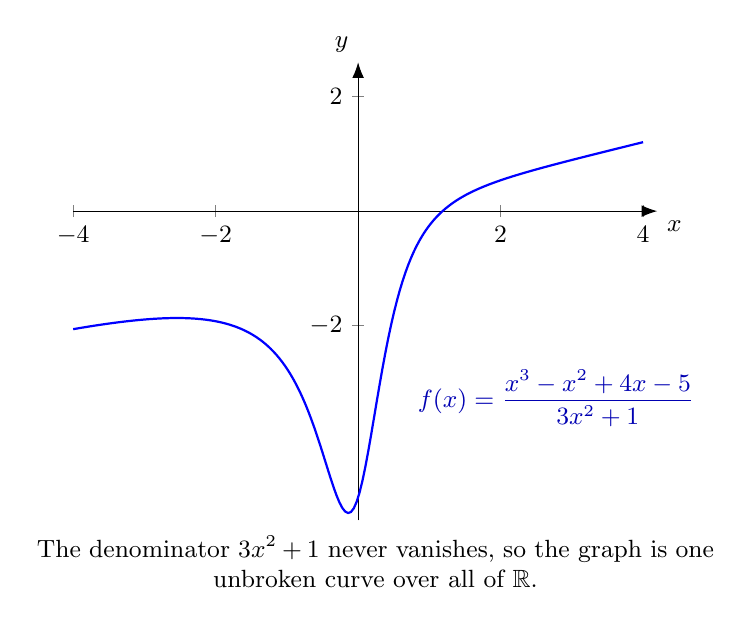
\begin{tikzpicture}[every node/.style={font=\small}]
	\begin{axis}[
		width=9cm, height=7.4cm,
		axis lines=middle, axis line style={-{Latex[length=2mm]}},
		xmin=-4, xmax=4.2, ymin=-5.4, ymax=2.6,
		xtick={-4,-2,2,4}, ytick={-2,2},
		tick label style={font=\small},
		xlabel={$x$}, ylabel={$y$},
		xlabel style={below right}, ylabel style={above left},
		samples=200, clip=false
		]
		\addplot[blue, thick, domain=-4:4] {(x^3-x^2+4*x-5)/(3*x^2+1)};
		\node[blue!70!black, anchor=north west, font=\small] at (axis cs:0.7,-2.6) {$f(x)=\dfrac{x^3-x^2+4x-5}{3x^2+1}$};
	\end{axis}
	\node[anchor=north, align=flush center, text width=8.6cm] at ([yshift=-2pt]current bounding box.south) {The denominator $3x^2+1$ never vanishes, so the graph is one unbroken curve over all of $\mathbb R$.};
\end{tikzpicture}
\end{document}
